%%-*-latex-*-

\documentclass[compress,dvipdfmx]{beamer}

\usepackage[english]{babel}
\usepackage{amssymb,amsmath}
\usepackage{xspace}
\usepackage{hyphenat}
%\usepackage{verbatim}

\setbeamertemplate{theorems}[numbered]
% Beamer configuration
%

\usefonttheme{default}
\usefonttheme{serif}
\usefonttheme{structurebold}

\setbeamersize{text margin left=6mm}
\setbeamersize{text margin right=6mm}
\setbeamertemplate{headline}{}
\setbeamertemplate{navigation symbols}{}
\setbeamertemplate{footline}[page number]{}
\setbeamertemplate{itemize items}[circle]
\setbeamertemplate{theorems}[numbered]

\leftskip=0pt
\rightskip=0pt


\newcommand\lang[1]{\texttt{#1}\xspace}
\newcommand\Java{\lang{Java}}
\newcommand\C{\lang{C}}
\newcommand\Lisp{\lang{List}}
\newcommand\Csharp{\lang{C\#}}
\newcommand\Haskell{\lang{Haskell}}
\newcommand\OCaml{\lang{OCaml}}

\frenchspacing  % Follow French conventions after a period

% ------------------------------------------------------------------------
% Document
%
\title{Introduction to Garbage Collection}
\author{Christian Rinderknecht}
\institute{Eszterházy Károly Katolikus Egyetem}
\date{September 2026}

\begin{document}

\frame{\maketitle}

\begin{frame}
  \frametitle{Garbage Collection}

  The runtimes of many programming languages feature \textbf{dynamic
    memory management}.

  \bigskip

  The first aspect of that management is \textbf{allocation}, that is,
  the program can create pieces of data (called in this context
  \textbf{objects}) whole lifetime can be that of the program
  itself. In particular, they can outlive the procedure or function
  that created them.

  \bigskip

  Those objects exist in a memory area called the \textbf{heap}. More
  precisely, a \textbf{continuous block} is allocated for one
  object, whose size depends on the \textbf{type} of the object.

\end{frame}

\begin{frame}[containsverbatim]
  \frametitle{Garbage Collection}

  For example, in \Java, we can declare a type for the cells
  in a linked list of integers as follows:
\begin{verbatim}
class Cell {
  int   content;
  Cell  next;
}
\end{verbatim}
Each cell contains an integer and a \textbf{pointer} to another
cell. The pointer is implicit in the recursive occurrence of the type
name \texttt{Cell}. It is either the address of an object in memory,
or a special value \textbf{nil} (noted \texttt{null} in
\Java). Consequently, each cell requires at least two
\textbf{words} (one for each field and perhaps more, depending on the
data layout).

\end{frame}

\begin{frame}[containsverbatim]
  \frametitle{Garbage Collection}

  A cell can be allocated with the built-in function \texttt{new},
  like so:
\begin{verbatim}
Cell c = new Cell ();
\end{verbatim}

A word is the smallest amount of memory that can be
addressed and filled by a primitive type or a pointer ---~64
bits in modern computers.

\bigskip

In other words, we can imagine memory as a table with addresses as
keys and words as values. Those values may be interpreted as another
key (address) or not (primitive type).

\bigskip

Then we can modify the contents of the fields it contains, as many
times as we wish to. Every call to \texttt{new} returns the
\textbf{address of a new block} drawn from the available memory.

\end{frame}

\begin{frame}[containsverbatim]
  \frametitle{Garbage Collection}

Because each allocation removes from available, finite memory, it is
necessary for the GC to \textbf{free the memory used by useless
  objects}, which it needs to define and find.

\bigskip

In some programming languages, like \C, this task is entirely
delegated to the programmers. They have a predefined procedure
\texttt{free} that frees a memory block:
\begin{verbatim}
free(c);
\end{verbatim}
After it is executed, the block pointed at by~\texttt{c} is considered
available again, so its address can be reused in a future
allocation.

\end{frame}


\begin{frame}[containsverbatim]
  \frametitle{Garbage Collection}

  \label{C_errors}

  In \C, the premature of an object may lead to errors:
  \begin{center}
    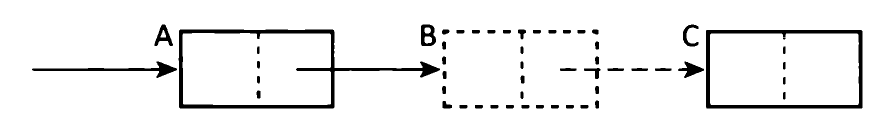
\includegraphics[width=0.5\textwidth]{wrong_free.png}
  \end{center}
  Here, \texttt{B} has been freed. The live object \texttt{A} now
  contains a \textbf{dangling pointer}, and the memory occupied by
  \texttt{C} has \textbf{leaked}: \texttt{C} is not reachable, but it
  cannot be freed.

  \bigskip

  Another common mistake is freeing an already freed object (like
  \texttt{B} above): this is an undefined behaviour and thus a source
  of \textbf{non\hyp{}determinism}.

\end{frame}


\begin{frame}
  \frametitle{Garbage Collection}

  In \Java, there is no equivalent to the \texttt{free} procedure of
  \C because the identifying and freeing of useless objects is left to
  the runtime system.

  \bigskip

  That part of the runtime is called the \textbf{garbage collector}
  (GC). At regular intervals, it interrups the program, analyses the
  heap, find out the useless objects and free them.

  \bigskip

  This technique was invented by McCarthy, creator of the functional
  programming language \Lisp in \oldstylenums{1960}. It is widely used
  in mainstream languages like \Java, \Csharp, \Haskell or \OCaml.

  \bigskip

  Beyond avoiding the two errors above, a GC may also free many
  objects at a time, which is more efficient than any sequential,
  manual deallocation.

\end{frame}

\begin{frame}
  \frametitle{Garbage Collection}

  How does a GC determine what objects are useless, since it has no
  access to the source code or the programmer (interactively)?

  \bigskip

  The GC can rely on the following condition:
  \begin{center}
    \it If, at a certain moment, a program does not have a pointer
    (anymore) to an object, that object is considered useless.
  \end{center}
  That condition is not true in \C, where pointers can be forged (type
  casting) from integers, but it holds in \Java for example.

  \bigskip

  Therefore, the memory block of that object can be reused for
  another, without the program being able to observe that reuse.

\end{frame}


\begin{frame}
  \frametitle{Garbage Collection}

  When a program has the address of an object, it is said to be
  \textbf{alive}, and \textbf{dead} otherwise.

  \bigskip

  We can define inductively the notion of liveness:
  \begin{definition}
    \it Both the global and local variables of the program are called
    \textbf{roots}. By definition (base case), the object pointed at
    by a root is alive. Moreover, if an object is alive and one of its
    fields contains the address of another object, then that latter
    object is alive too (inductive case).
  \end{definition}

  \medskip

  What counts as global and local variable depends on the programming
  language. In \Java, the former are the \texttt{static} fields
  (a.k.a. instance fields), and the latter are methods arguments
  (including \texttt{this}) and the variables declared in the method
  being executed.

  \end{frame}


\begin{frame}
  \frametitle{Garbage Collection}

  The heap can now be seen as a \textbf{graph}, where the
  \textbf{vertices} correspond to the roots and the objects, and the
  \textbf{edges} model the pointers between objects (that is, if one's
  block contains a pointer to another's).

  \bigskip

  The live objects are then the vertices \textbf{reachable from the
    roots}.

  \bigskip

  Therefore, to determine the live objects at a given time, the GC has
  to traverse the graph of objects from the roots.

\end{frame}


\begin{frame}
  \frametitle{Garbage Collection}

  \begin{center}
    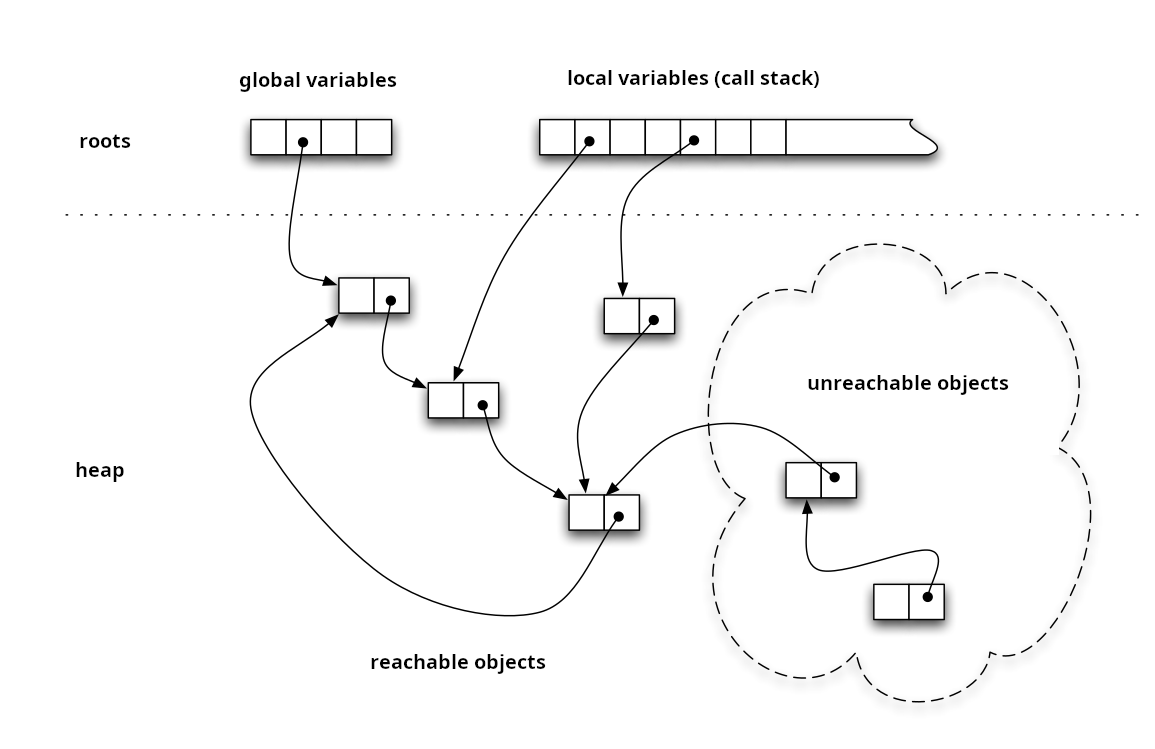
\includegraphics[width=\textwidth]{memory.png}
  \end{center}

\end{frame}


\begin{frame}
  \frametitle{Garbage Collection}

  We started this introduction by referring to `useful objects', but
  now we see that the appropriate concept is that of `live objects',
  which is the same as `reachable objects'.

  \bigskip

  It is obvious that all dead objects are useless, but the reciprocal
  is not true: a live object might be useless if the program does
  nothing with it. They are allocated in the heap but cannot be
  reclaimed. This is a case of \textbf{memory leak}. (We saw
  page~\pageref{C_errors} another case of memory leak in \C.)

\end{frame}

\end{document}
